\chapter{Inéquations du premier degré}

\section{Notions ensemblistes}

Pour écrire les réponses de ce chapitre, nous aurons besoin d'une notation particulière liée aux ensembles. Comme nous l'avons déjà vu, on note $\R$ l'ensemble de tous les nombres réels (nombres entiers et à virgule, positifs et négatifs). Un intervalle est un sous-ensemble de $\R$, c'est-à-dire une partie de cet ensemble.

\begin{definition}
On note 
$$
[a;b]
$$
l'ensemble qui contient tous les nombres entre $a$ et $b$, avec $a$ et $b$ compris dans cet ensemble. Ce genre d'intervalle avec des crochets qui pointent vers l'intérieur est appelé \emph{intervalle fermé}.
\index{intervalle!fermé}
\end{definition}

Par exemple, l'intervalle $[-2;4]$ contient $-1$, $0$, $0.2431423$ ainsi que $-2$~et~$4$. 

\begin{definition}
On note 
$$
]a;b[
$$
l'ensemble qui contient tous les nombres entre $a$ et $b$, avec $a$ et $b$ \textbf{n'étant pas compris} dans cet ensemble. Ce genre d'intervalle avec des crochets qui pointent vers l'extérieur est appelé \emph{intervalle ouvert}.\index{intervalle!ouvert}
\end{definition}

Par exemple, l'intervalle $]0;5[$ contient $1$, $2$, $3$, $\pi$, $4.99999999$ mais ni~$5$~ni~$0$. 

\begin{definition}\index{infini}
On appelle \emph{plus infini} le nombre plus grand que n'importe quel autre et on le note
$$
+\infty
$$
réciproquement, on appelle \emph{moins infini} le nombre plus petit que n'importe quel autre et on le note
$$
-\infty
$$
\end{definition}

Ainsi, certains intervalles utilisent cette notion d'infini, par exemple si l'on veut prendre tous les nombres plus grands que $42$, sans le nombre $42$ lui-même, on va noter
$$
]42;+\infty[
$$

\begin{remarque}
Certains ensembles ne sont ni ouverts, ni fermés. Par exemple
$$
]-2;2]
$$
Contient tous les nombres compris entre $-2$ et $2$, sans le $-2$ mais avec le $2$.
\end{remarque}

\section{Symboles}

Les symboles d'inéquations se lisent toujours de gauche à droite. On peut trouver les quatre symboles suivants :

\hspace{5mm}\index{Inéquation!symboles}

\shadowbox{
\begin{tabular}{ll|ll}
$<$ & strictement plus petit que & $>$ & strictement plus grand que\\
$\leq$ & plus petit ou égal à & $\geq$ & plus grand ou égal à\\
\end{tabular}
}

\hspace{5mm}

Ainsi l'inéquation suivante 
$$
x \geq 6
$$
se lit : "$x$ est plus grand ou égal à $6$".

\section{À une inconnue}

Contrairement à une équation, une inéquation ne va pas nous donner une valeur bien précise pour $x$, mais un ensemble de valeurs qui satisfait l'inégalité. Par exemples pour l'inéquation
$$
2x-3 \leq x+1
$$
la valeur $\textcolor{red}{x=1}$ fait partie de l'ensemble des solutions car $2\cdot \textcolor{red}{1} -3 = -1$, $\textcolor{red}{1}+1 = 2$ et on a bien $-1\leq 2$. Par contre la valeur $\textcolor{blue}{x=5}$ n'en fait pas partie car $2\cdot \textcolor{blue}{5} -3 = 7$, $\textcolor{blue}{5}+1 = 6$ et on n'a pas $7\leq 6$.

\subsection{Résolution d'une inéquation}

La résolution d'une équation à une inconnue se fait comme une résolution d'une équation à une inconnue à la différence que si l'on doit multiplier ou diviser des deux côtés par un nombre négatif, on inverse le sens de l'inégalité.

\begin{exemple}
Résoudre l'inéquation suivante :
$$
2x-3 \leq x+1
$$
On va utiliser les mêmes outils que pour les équations :
$$
\begin{array}{lcll}
2x-3 &\leq& x+1 &\ssi^{-x} \\
x-3 &\leq & 1 &\ssi^{+3}\\
 x & \leq & 4&\\.
\end{array}
$$
On peut alors représenter en vert la solution sur la droite des réels :

\begin{center}
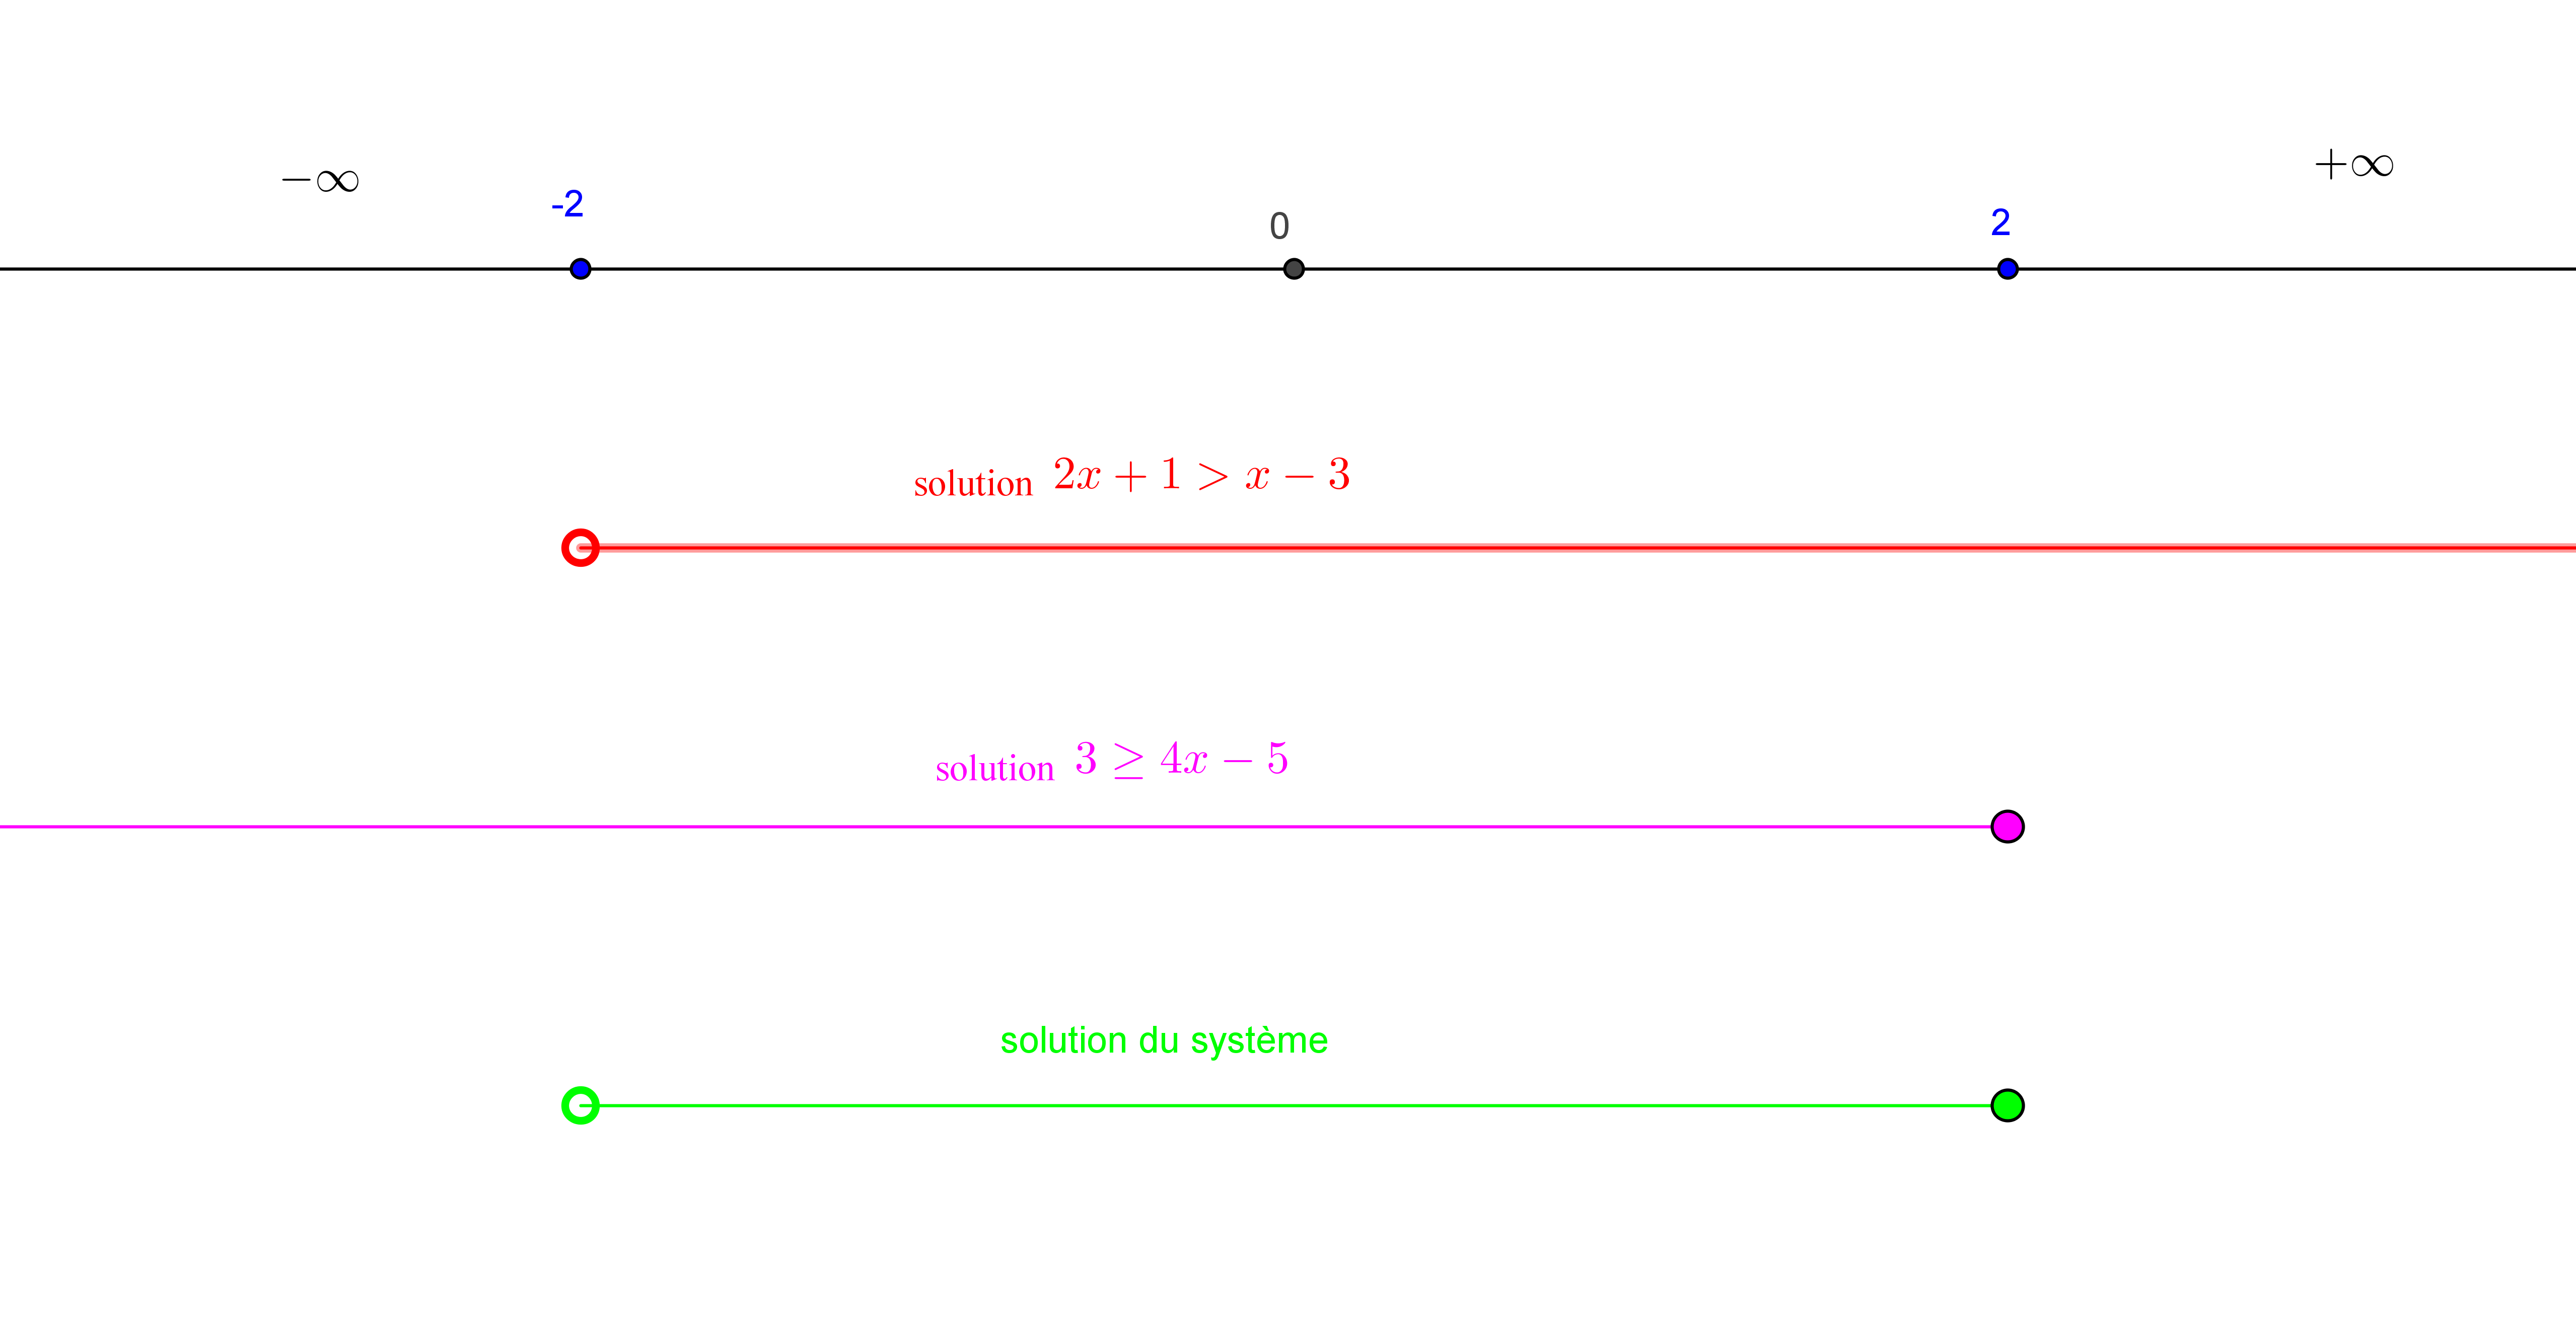
\includegraphics[width = 0.9\textwidth]{inequation1/innequation1.png}
\end{center}

Avec la convention suivante : si $x$ peut être égal au nombre, on remplit le point et si $x$ ne peut pas être égal, on laisse un rond vide. Pour savoir de quel côté part la demi-droite, il suffit d'essayer avec $x=0$ (ou un autre nombre). Si le test est concluant, on prend le côté où se trouve $0$, sinon l'autre. Dans notre exemple, $x\leq 4$ donc on a pris le côté du $0$.\index{Inéquation!solution graphique}

La solution du système est donc notée sous forme d'intervalle~\index{intervalle}
$$
S = ]-\infty ; 4]
$$
et se lit de la manière suivante "les solutions sont entre $-\infty$ et $4$ compris".

\end{exemple}

\subsection{Résolution d'un système d'inéquations}

Pour un système d'inéquations à une inconnue, la méthode est assez simple : il faut résoudre chaque inéquation séparément et représenter chaque solution sur la même droite des réels. La solution du système est alors à l'intersection des solutions, c'est-à-dire là où l'on trouve toutes les couleurs.

\begin{exemple}

Résoudre le système 
$$
\left\{
\begin{array}{lcl}
2x+1&>&x-3\\
3&\geq & 4x-5\\ 
\end{array}
\right.
$$
On résout chaque inéquation séparément et on trouve
$$
\left\{
\begin{array}{lcl}
x&>&x-2\\
2&\geq & x\\ 
\end{array}
\right.
$$

On représente ensuite la solution
\begin{center}
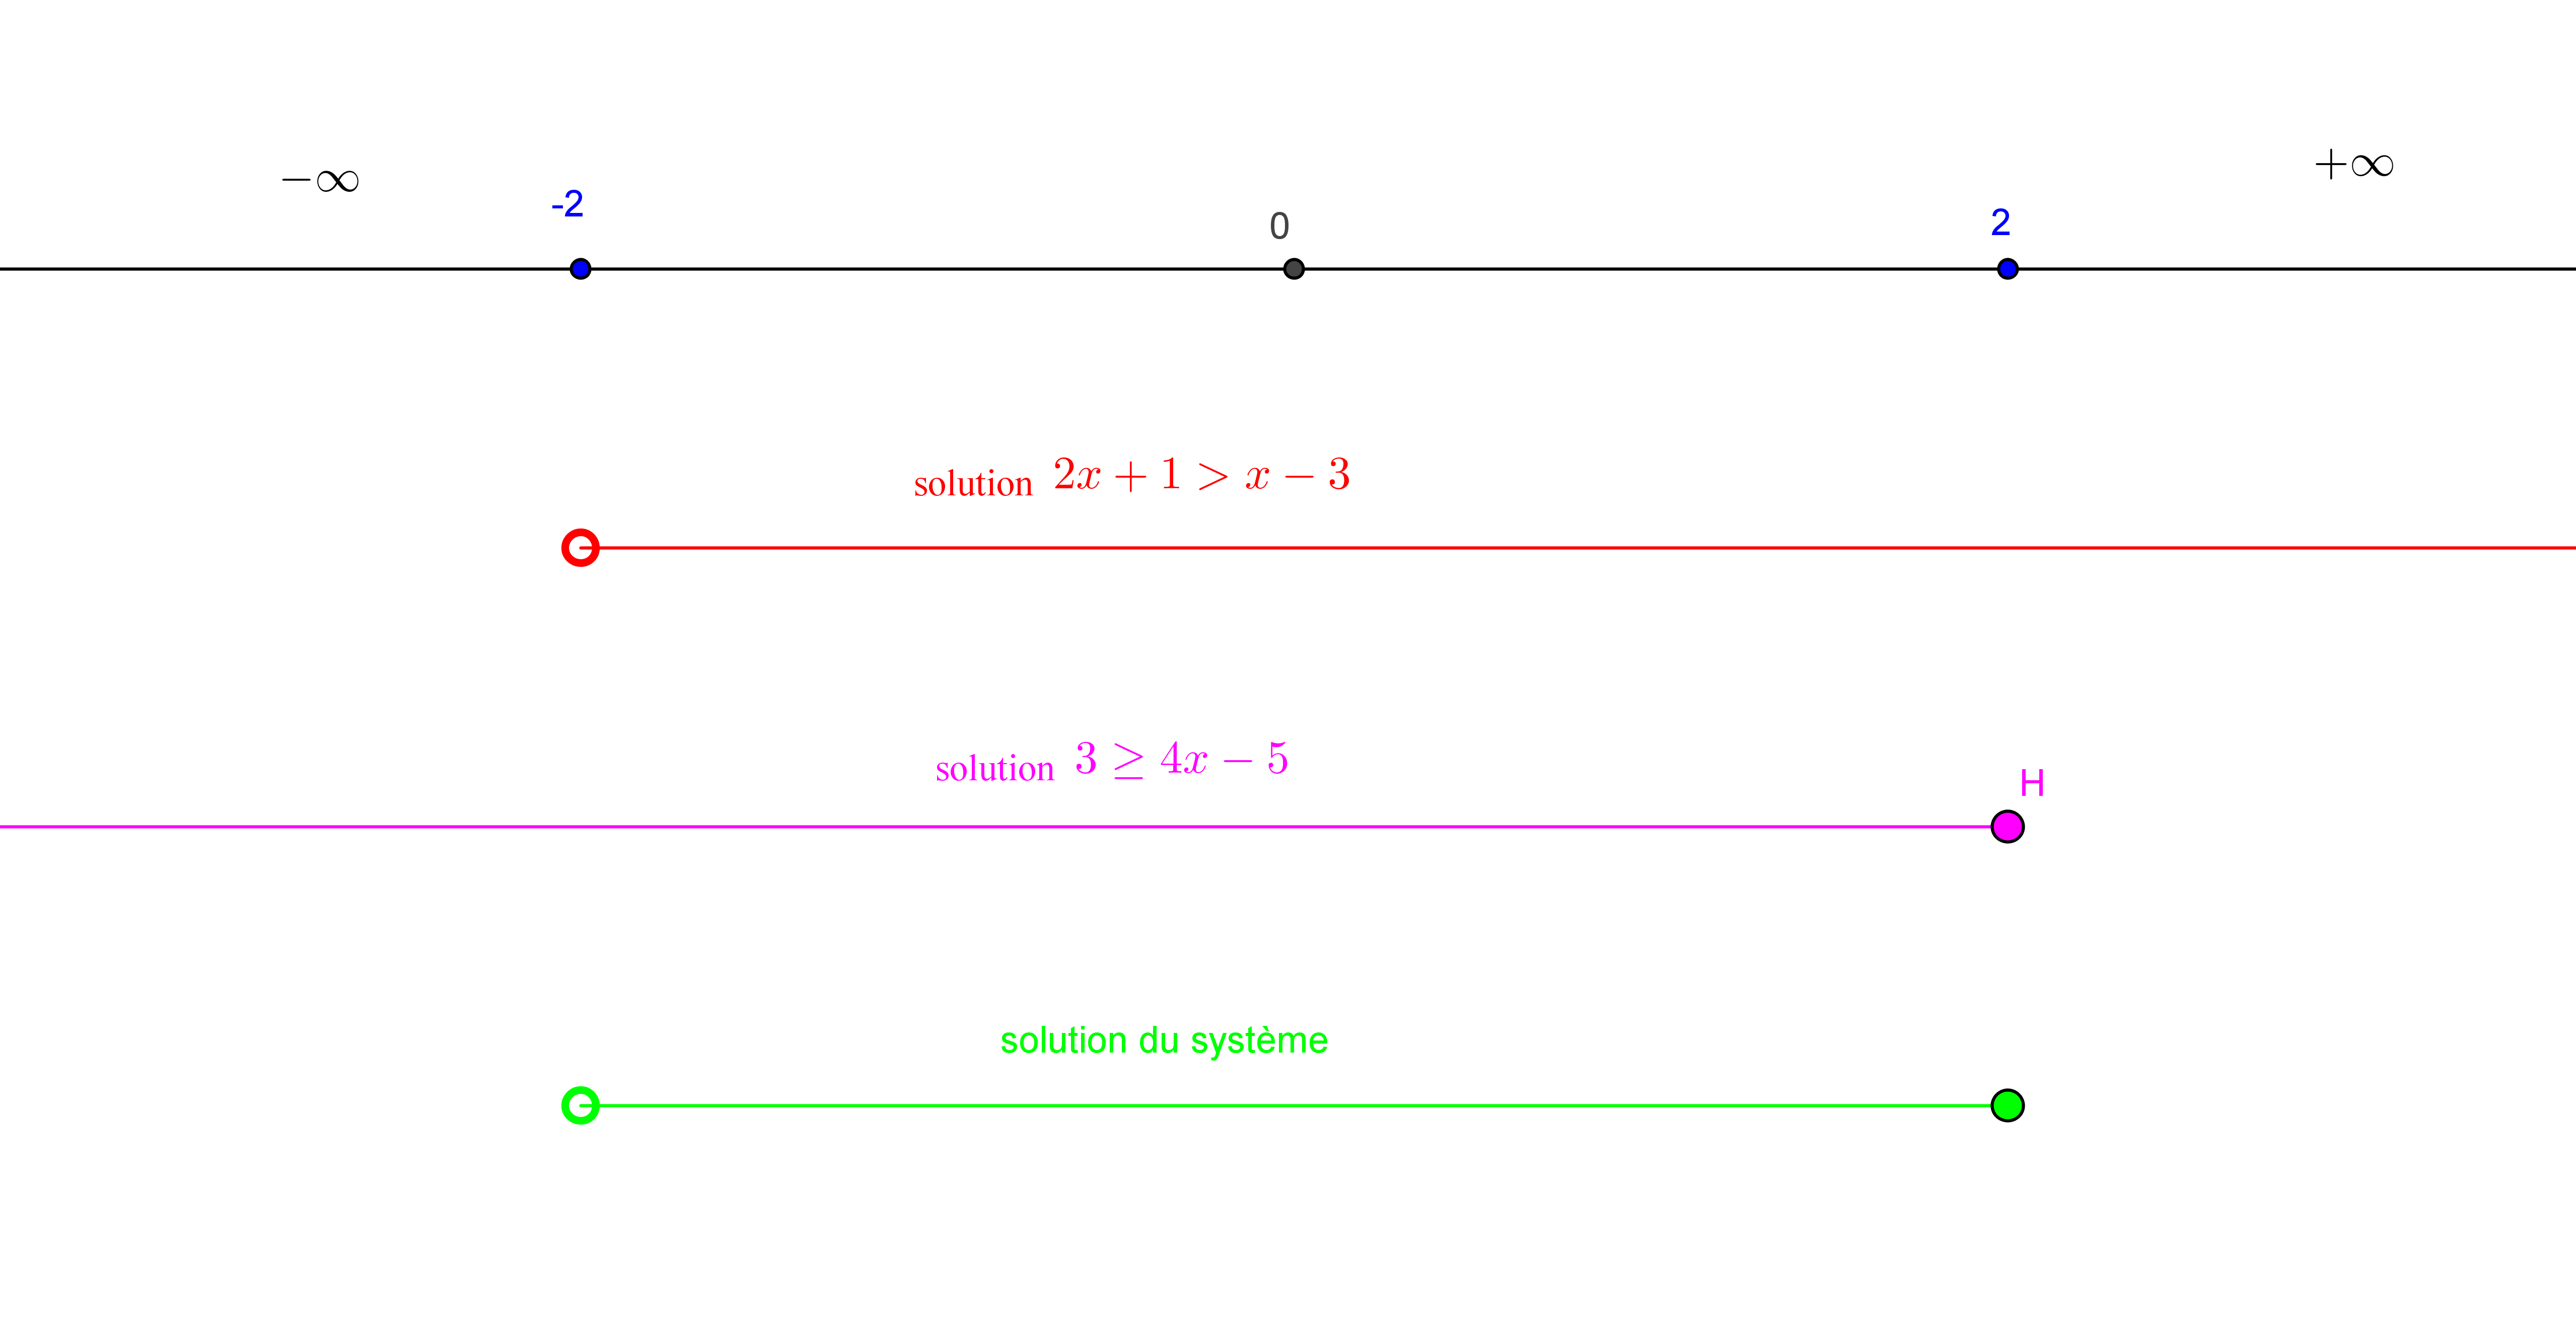
\includegraphics[width = 0.9 \textwidth]{inequation1/inequations1.png}
\end{center}
\end{exemple}

L'ensemble des solutions du système est donc donné par l'intervalle :
$$
S=]-2;2]
$$

\section{À plusieurs inconnues}

Cette section traite des inéquations à plusieurs inconnues. Nous n'aborderons que l'aspect graphique des solutions (comment représenter les solutions possibles) et donc par souci de représentation, nous ne traiterons que les inéquations à deux inconnues. Cependant, la notion se généralise facilement aux équations à trois, quatre, etc. inconnues.

\subsection{Résolution d'une inéquation}

Nous nous intéressons à la manière de représenter sur le plan une inéquation à deux inconnues. Elles sont du type
$$
ax+by \lessgtr c
$$

Regardons dans un premier temps comment représenter l'équation
$$
ax+by=c
$$
sur le plan. Il s'agit d'une équation du premier degré à deux inconnues. Une telle notion a déjà été abordée au chapitre~\ref{droite_plan}; il s'agit d'une droite dans le plan. Pour la représenter, il faut simplement trouver deux points qui sont sur la droite, par exemple en remplaçant $x$ par un nombre puis en déterminant la valeur de $y$ et réciproquement.

Cette droite va couper le plan en deux parties. Puisqu'il s'agit d'une inéquation, l'un des deux parties va vérifier l'inégalité et l'autre non. On peut donc prendre un point qui n'est pas sur la droite pour tester s'il fait partie de la solution. S'il en fait partie, on prendra son côté du plan, sinon, l'autre côté. On appelle cela le \emph{principe du tiers exclu}.\index{principe du tiers exclu}

\begin{exemple}
Résoudre graphiquement l'inéquation
\begin{eqnarray}
x-2y \geq 6 \label{inequation}
\end{eqnarray}
Commençons par représenter la droite 
$$
x-2y=6
$$
Il faut donc trouver deux points sur la droite. Usuellement on va remplacer une fois $x$ par $0$ et une fois $y$ par $0$, mais on peut choisir d'autres nombres ou remplacer deux fois $x$ ou deux fois $y$. Ainsi
$$
\begin{array}{lcl}
\textcolor{red}{x=0} &\Longrightarrow & 0-2y=6 \ssi \textcolor{red}{y=-3}\\
\textcolor{blue}{y=0} &\Longrightarrow & x-2\cdot 0 = 6 \ssi \textcolor{blue}{x = 6}
\end{array}
$$
La droite passe donc par les points $\textcolor{red}{(0;-3)}$ et $\textcolor{blue}{(6;0)}$.

Il faut maintenant tester un point. Usuellement, on teste le point $(0;0)$, mais on peut prendre un autre. Remplaçons $x$ et $y$ par $0$ dans l'inéquation~\ref{inequation}. On obtient
$$
0-2\cdot 0 \geq 6
$$
Or cette inégalité est fausse, donc le point $(0;0)$ ne fait pas partie de la solution. Le principe du tiers exclu nous indique qu'il faut prendre l'autre partie du demi-plan :
\begin{center}
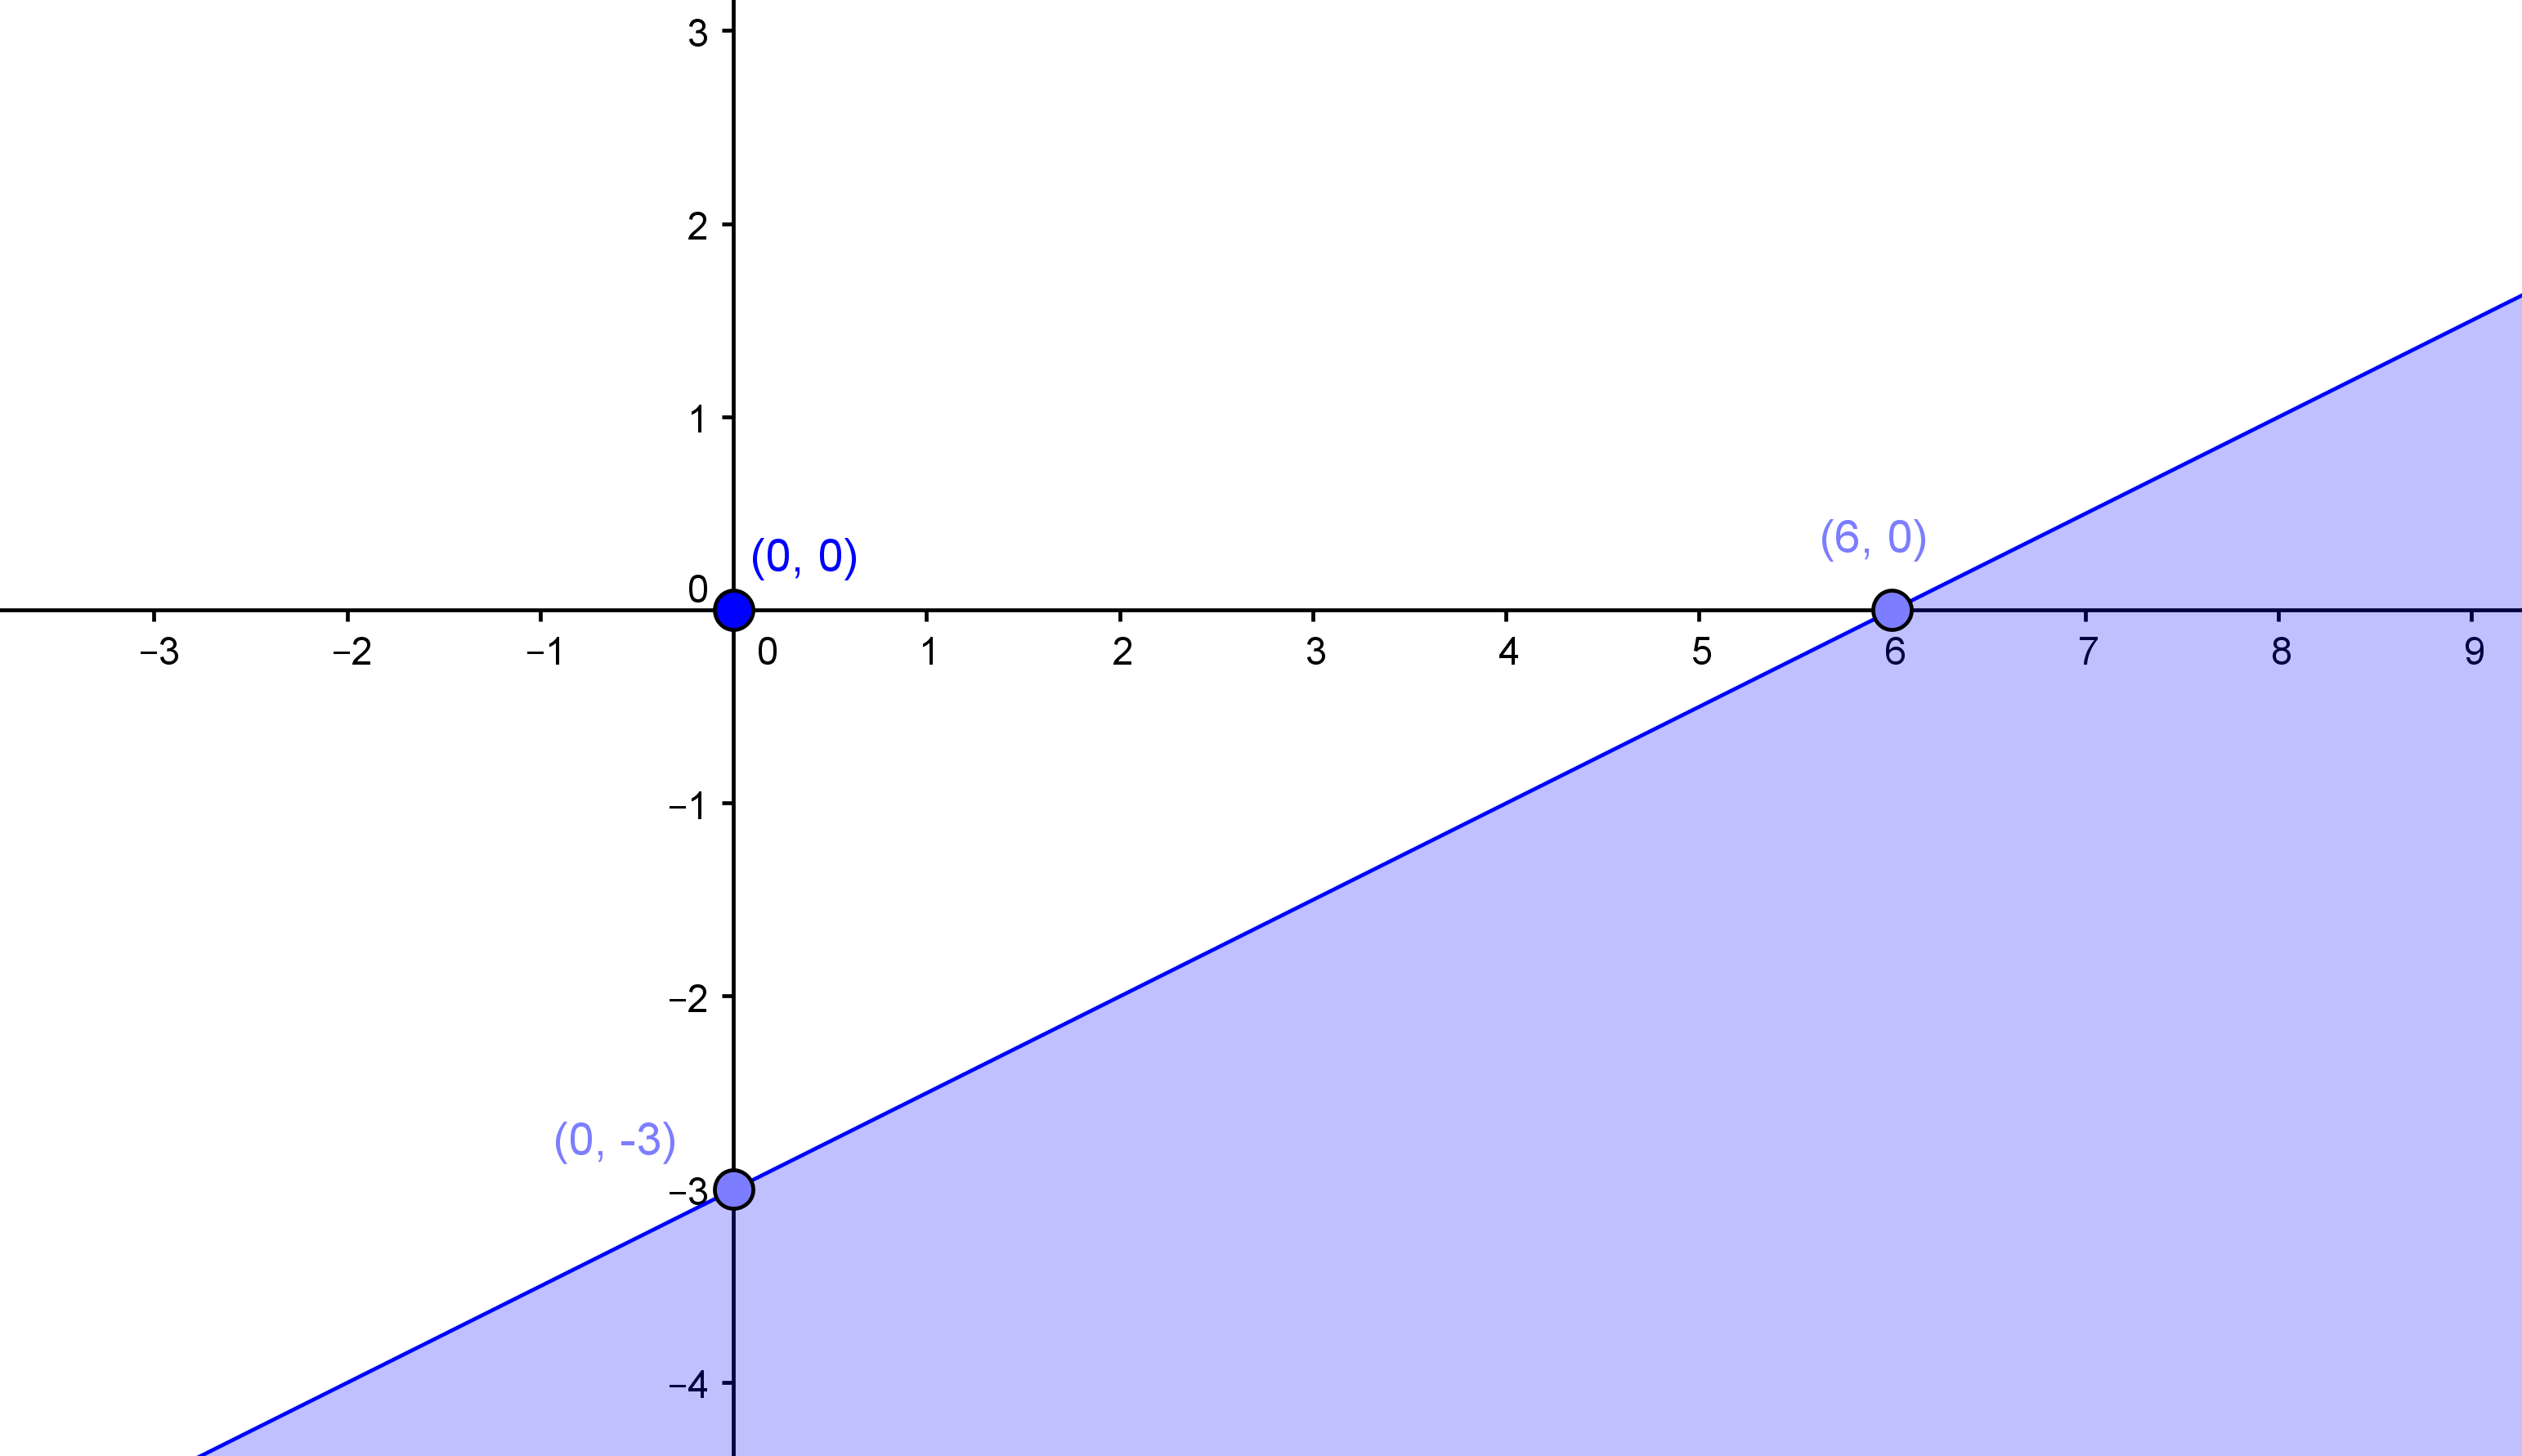
\includegraphics[width = 0.9\textwidth]{inequation1/inequation2.png}
\end{center}
\end{exemple}
\begin{remarque}
Par convention, si le symbole est une inégalité stricte ($>$ ou $<$), on va dessiner la droite en trait tillé, et sinon ($\leq$ ou $\geq$) on passera la droite en gras.
\end{remarque}

\subsection{Résolution d'un système d'inéquations}

Pour résoudre un système d'inéquations, on va résoudre graphiquement chaque inéquation sur le même système d'axes. La solution du système est là où se rejoignent les solutions de chaque inéquation.

\begin{exemple}
Résoudre graphiquement le système d'inéquations 
$$
\left\{
\begin{array}{lcl}
x-2y &\geq & 6\\
2x-4y & < & -6\\
\end{array}
\right.
$$
La solution est représentée par 
\begin{center}
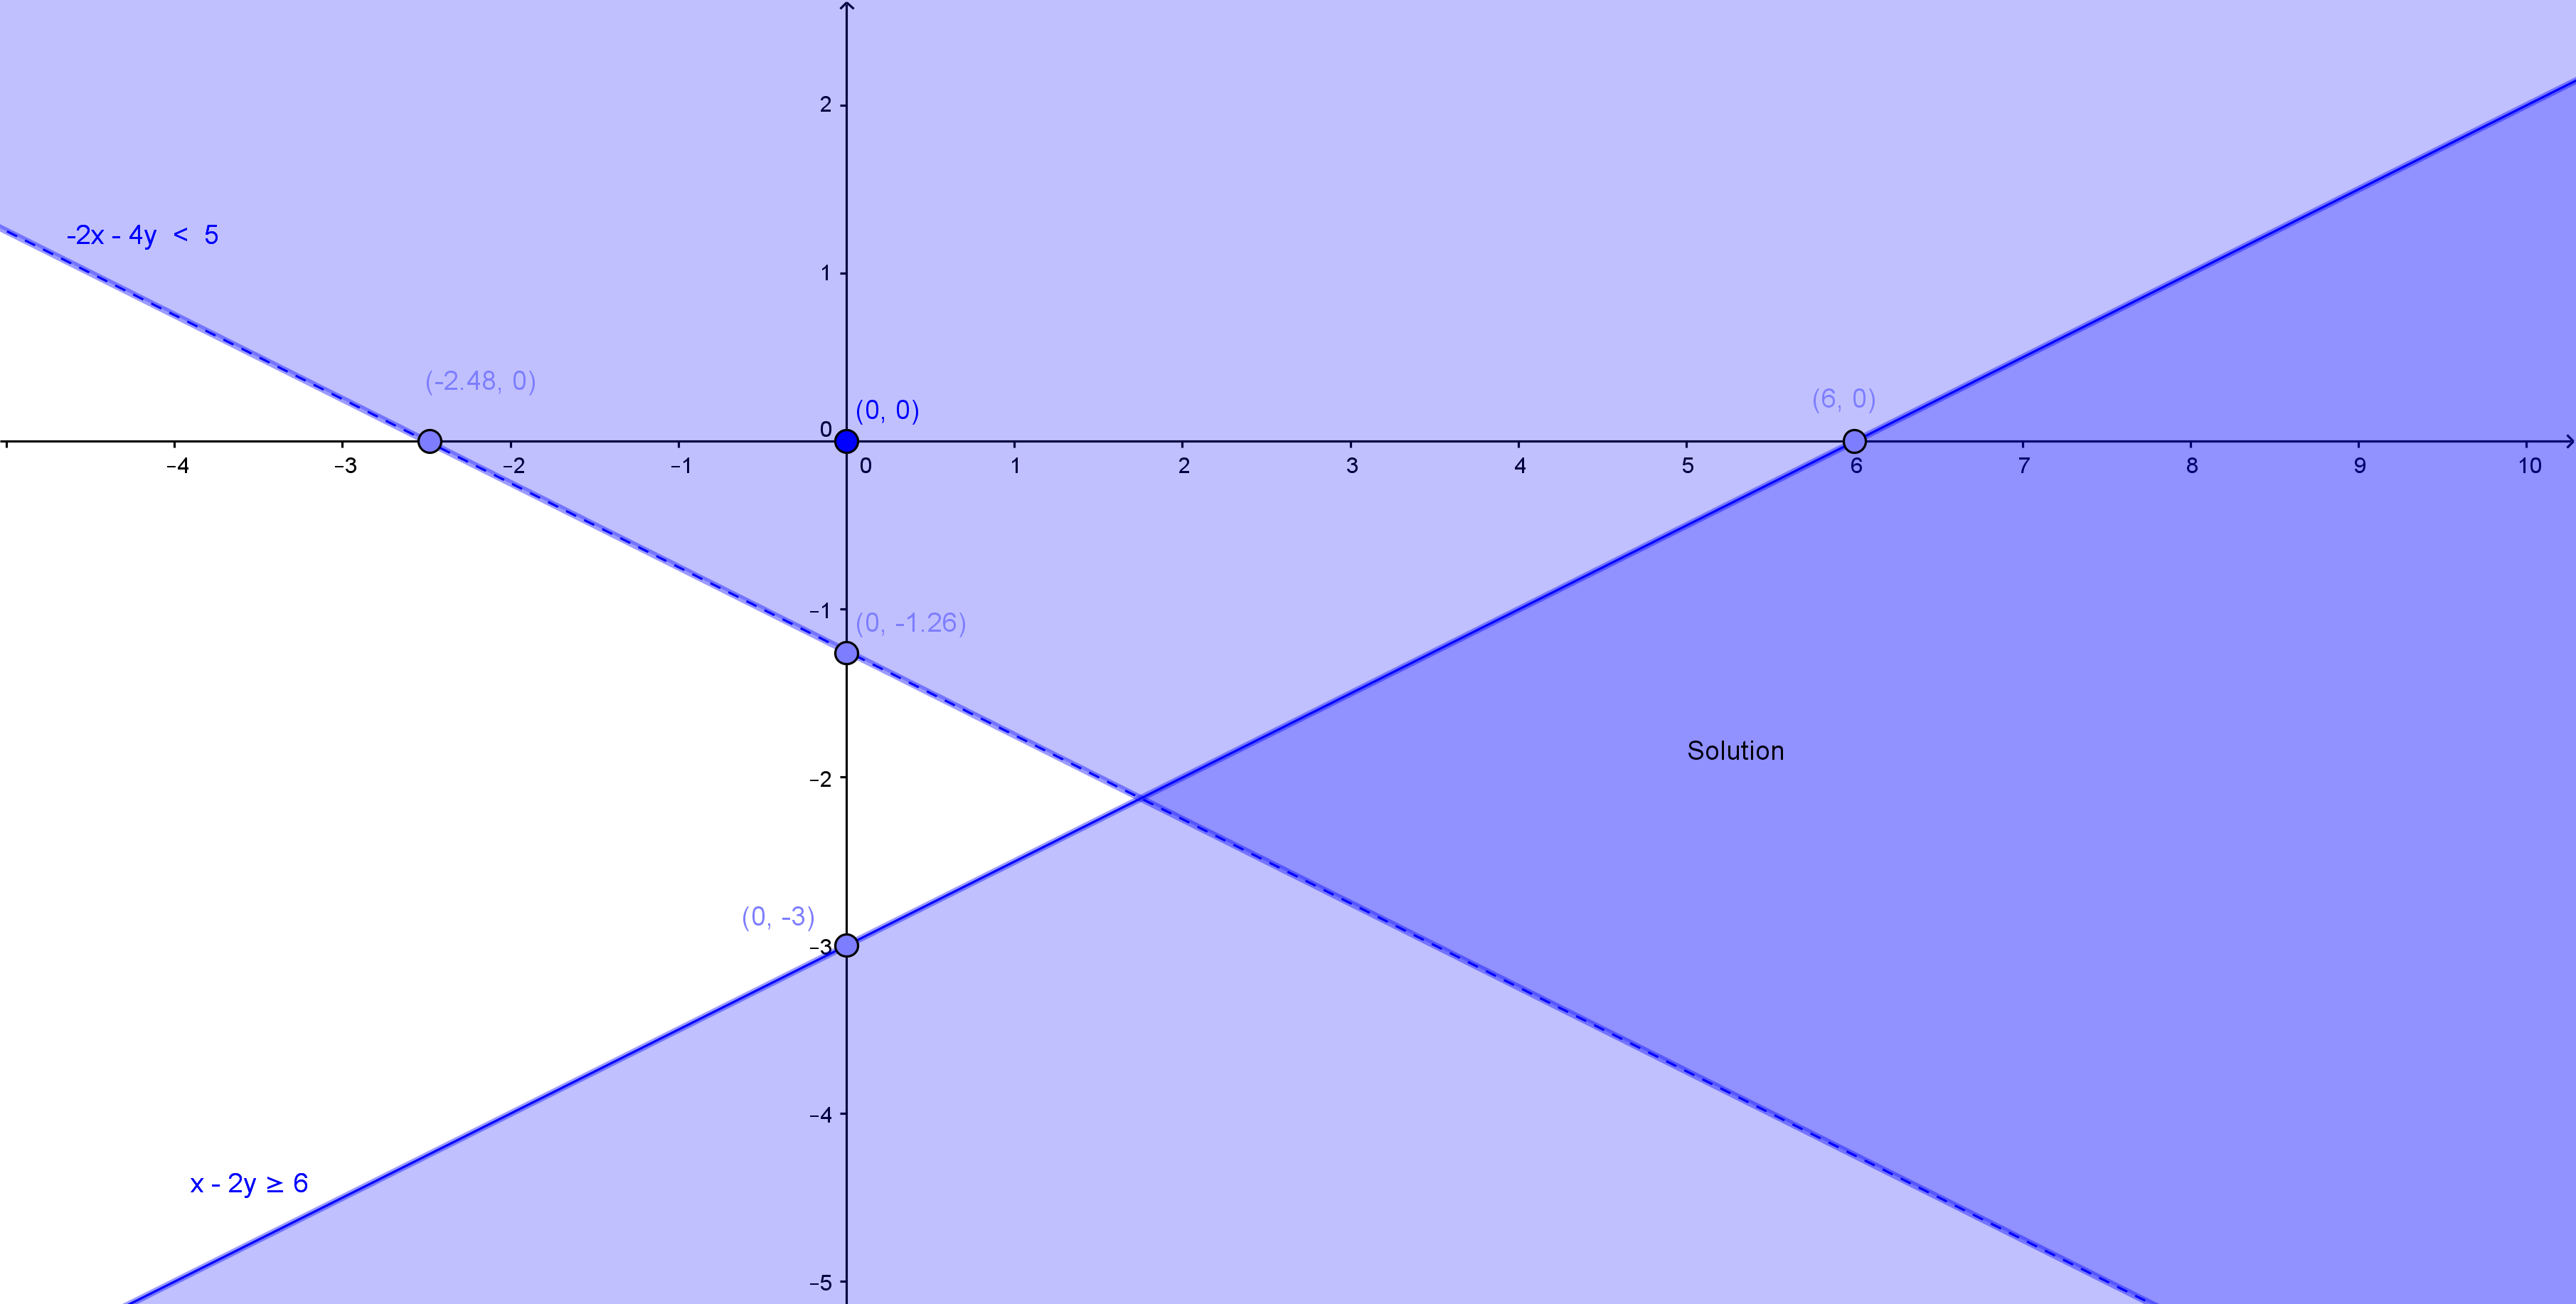
\includegraphics[width=0.9\textwidth]{inequation1/inequation21.png}
\end{center}
\end{exemple}

\begin{remarque}
On peut aussi représenter des solutions d'inéquations à trois inconnues :
$$
\left\{
\begin{array}{lcl}
3x + 2y - 4z &<& 2\\
x - 3y + 4z &\geq & -1\\
-2x - 3y - z &>& 4 \\
\end{array}
\right.
$$
\begin{center}
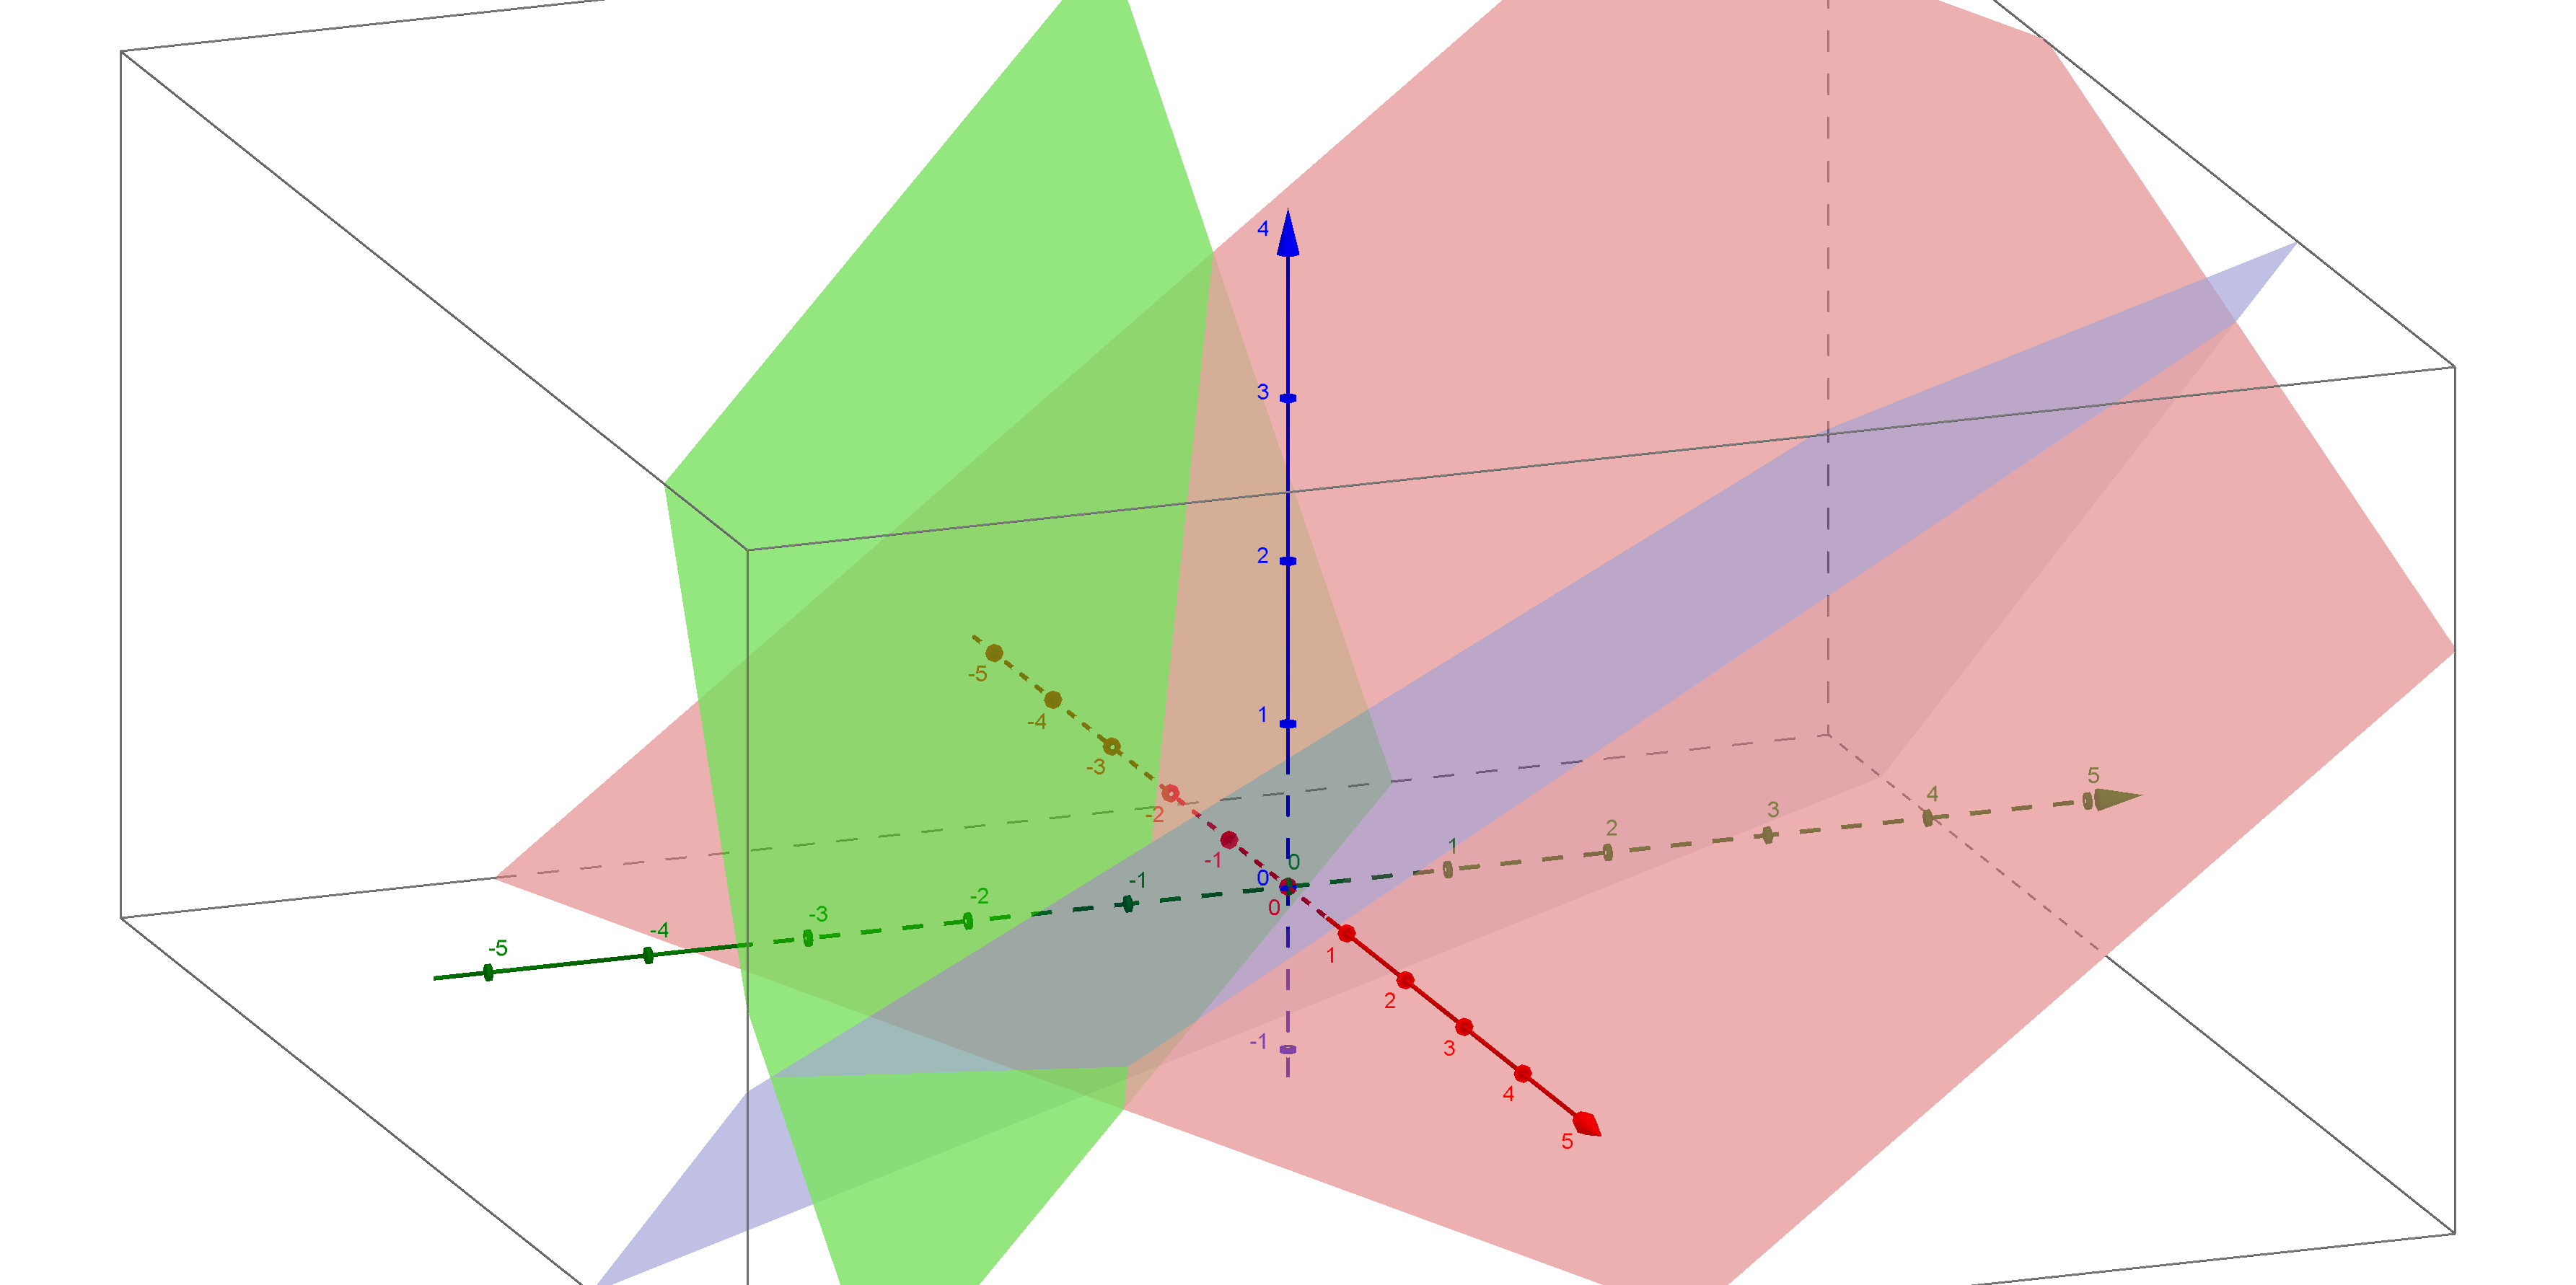
\includegraphics[width = 0.9\textwidth]{inequation1/inequation3.png}
\end{center}
Mais ça devient vite très compliqué.
\end{remarque}

\section{Exercices}

\begin{exercice}
Résoudre les inéquations du 1er degré suivantes :
\begin{multicols}{2}
\begin{enumerate}
\item $7x-6>5+6x$
\item $12-5x>x-60$
\item $\frac{x}{3}+\frac{x}{2}>\frac{x}{4}+\frac{1}{2}$
\item $\frac{x}{2}+4>\frac{2x}{3}-\frac{x}{8}$
\item $4\left( 5+x \right)>5\left( x+3 \right)$
\item $3-4(5-x)\le 2x+5$
\item $\frac{3x-1}{5}-\frac{13}{2}\ge \frac{7x}{3}-\frac{11\left( x+3 \right)}{6}$
\item $\frac{2x}{5}-\frac{2x-17}{3}<10-\frac{2x-6}{2}$
\item $4({{x}^{2}}+1)+8(3x-4)>4{{x}^{2}}$
\item $\frac{x-5}{3}-\frac{x-8}{4}\le 0$
\item $\frac{5x}{3}+1-\frac{8x+1}{4}>0$
\item $\frac{3x}{2}-\frac{2x}{3}\ge 5\left( \frac{x}{6}+1 \right)-5$
\item $\frac{3x}{2}-\frac{2x}{3}>5\left( \frac{x}{6}+1 \right)-5$
\item $\left( 3x+45 \right)\left( 3x+3 \right)<\left( 3x+6 \right)\left( 3x+18 \right)$
\item $\frac{6x-1}{12}-\frac{3}{4}\ge 4x-\frac{5\left( 1-4x \right)}{2}$
\item $2x-\frac{6x+1}{2}-\frac{8x-1}{3}+\frac{11x}{3}<0$
\item $\frac{\left( 3x-7 \right)\left( 3x+7 \right)}{6}<\frac{{{\left( x-2 \right)}^{2}}}{2}+\frac{{{\left( 2x+1 \right)}^{2}}}{4}$
\item $2x-\frac{2x}{9}\le \frac{1}{9}\left( 16x-\frac{3}{2} \right)$
\item $\frac{-x+1}{3}-\frac{-x-1}{4}\ge -\frac{x}{2}+\frac{2+x}{24}$
\item $\frac{{{\left( x+1 \right)}^{2}}}{16}-\frac{1+x}{2}<\frac{{{\left( x-1 \right)}^{2}}}{16}-\frac{2+x}{4}$
\end{enumerate}
\end{multicols}
\end{exercice}

\begin{exercice}
Résoudre les systèmes d'inéquations du premier degré suivants :
\begin{multicols}{2}
\begin{enumerate}
\item $\left\{ \begin{matrix}
   7x+3>0  \\
   5x-9\le 0  \\
\end{matrix} \right.$
\item $\left\{ \begin{matrix}
   -11x+5<0\,\,\,\,\,\,\,\,\,\,\,  \\
   5\left( 1+4x \right)\ge 7+2x  \\
\end{matrix} \right.$
\item $\left\{ \begin{matrix}
   -x-2\le 0\,\,\,\,\,\,\,\,\,\,\,\,\,\,\,  \\
   -2x+\frac{x}{2}+1\ge -\frac{x}{4}  \\
   \frac{15x-4}{2}<1+6x\,\,\,  \\
\end{matrix} \right.$
\item $\left\{ \begin{matrix}
   8x-7\ge \frac{15x-9}{2}  \\
   4x-5>5x-\frac{8}{3}\,\,  \\
\end{matrix} \right.$
\item $\left\{ \begin{matrix}
   2(4x+1)\ge 5x+8\,\,\,\,\,\,\,\,\,  \\
   2(3x+2)>5(3x-10)  \\
\end{matrix} \right.$
\item $\left\{ \begin{matrix}
   8x+\frac{14x}{5}\ge 66-\frac{12x}{5}  \\
   \frac{1}{6}\left( \frac{7x}{4}+x \right)>x-\frac{13}{2}  \\
\end{matrix} \right.$
\item $\left\{ \begin{matrix}
   5(20-x)>3x+68  \\
   3(x-7)<4(5x-1)  \\
\end{matrix} \right.$
\item $\left\{ \begin{matrix}
   \frac{2x-7}{4}-\frac{x+1}{8}\ge \frac{x-5}{2}\,\,\,\,\,\,\,  \\
   \frac{3x-14}{12}+\frac{3x-2}{4}\ge \frac{2x-1}{3}  \\
\end{matrix} \right.$
\end{enumerate}
\end{multicols}
\end{exercice}
 
\begin{exercice}
Résoudre graphiquement les inéquations à deux inconnues suivantes :
\begin{multicols}{3}
\begin{enumerate}
\item $3x+y\le 9$
\item $2x-5y>10$
\item $-2x+7y>4$
\item $4x+3y\ge -8$
\item $3y<18$
\item $-5x\le 25$
\end{enumerate}
\end{multicols}
\end{exercice}


\begin{exercice}
Résoudre graphiquement les systèmes d'inéquations à deux inconnues suivants :
\begin{multicols}{3}
\begin{enumerate}
\item $\left\{ \begin{matrix}
   -3x+4y\le 12  \\
   2x+y<8\,\,\,\,\,\,\,  \\
\end{matrix} \right.$
\item $\left\{ \begin{matrix}
   x+y\ge 2  \\
   y>3\,\,\,\,\,\,\,\,  \\
   x\le 4\,\,\,\,\,\,\,\,  \\
\end{matrix} \right.$
\item $\left\{ \begin{matrix}
   3x+6y\le 18  \\
   3x-6y\le 18  \\
   -3x+6y\le 18  \\
   -3x-6y\le 18  \\
\end{matrix} \right.$
\end{enumerate}
\end{multicols}
\end{exercice}

\section{Corrigés}

\begin{solution}
Résoudre les inéquations du 1er degré suivantes : 
\begin{multicols}{3}
\begin{enumerate}
\item $x>11$	
\item $x<12$
\item $x>\frac{6}{7}$	
\item $x<96$	
\item $x<5$
\item $x\le 11$
\item $x\ge 12$
\item $x<10$
\item $x>\frac{7}{6}$
\item $x\le -4$
\item $x<\frac{9}{4}$
\item $S=\mathbb{R}$
\item $S=\varnothing $
\item $x<-\frac{3}{8}$
\item $x\le \frac{10}{81}$
\item $S=\mathbb{R}$
\item $x<\frac{125}{12}$
\item $S=\varnothing $
\item $x\ge -\frac{4}{3}$
\item $S=\varnothing $
\end{enumerate}
\end{multicols}
\end{solution}

\begin{solution}
Résoudre les systèmes d'inéquations du 1er degré suivants : 
\begin{enumerate}
\item $\left\{ \begin{array}{ll}
  & x>-\frac{3}{7}\  \\ 
 & x\le \frac{9}{5}\  \\ 
\end{array} \right.\ \ \ S=\left\{ x\left| -\frac{3}{7}<x\le \frac{9}{5} \right. \right\}\ \ ou\ \ x\in \left] -\frac{3}{7}\ ;\ \frac{9}{5} \right]\ $	
\item $\left\{ \begin{array}{ll}
  & x>\frac{5}{11} \\ 
 & x\ge \frac{1}{9} \\ 
\end{array} \right.\ \ \ \ S=\left\{ x\left| x>\frac{5}{11} \right. \right\}\ \ ou\ \ x\in \left] \frac{5}{11}\ ;\ +\infty  \right[$	
\item $\left\{ \begin{array}{ll}
  & x\ge -2 \\ 
 & x\le \frac{4}{5} \\ 
 & x<2 \\ 
\end{array} \right.\ \ \ \ S=\left\{ x\left| -2\le x\le \frac{4}{5} \right. \right\}\ \ ou\ \ x\in \left[ -2\ ;\ \frac{4}{5} \right]$	
\item $\left\{ \begin{array}{ll}
  & x\ge 5 \\ 
 & x<-\frac{7}{3} \\ 
\end{array} \right.\ \ \ \ S=\varnothing $	
\item $\left\{ \begin{array}{ll}
  & x\ge 2 \\ 
 & x<6 \\ 
\end{array} \right.\ \ \ \ S=\left\{ x\left| 2\le x<6 \right. \right\}\ \ ou\ \ x\in \left[ 2\ ;\ 6 \right[$
\item $\left\{ \begin{array}{ll}
  & x\ge 5 \\ 
 & x<12 \\ 
\end{array} \right.\ \ \ \ S=\left\{ x\left| 5\le x<12 \right. \right\}\ \ ou\ \ x\in \left[ 5\ ;\ 12 \right[$
\item $\left\{ \begin{array}{ll}
  & x<4 \\ 
 & x>-1 \\ 
\end{array} \right.\ \ \ \ S=\left\{ x\left| -1<x<4 \right. \right\}\ \ ou\ \ x\in \left] -1\ ;\ 4 \right[$
\item $\left\{ \begin{array}{ll}
  & x\le 5 \\ 
 & x\ge 4 \\ 
\end{array} \right.\ \ \ \ S=\left\{ x\left| 4\le x\le 5 \right. \right\}\ \ ou\ \ x\in \left[ 4\ ;\ 5 \right]$
\end{enumerate}
\end{solution}

\begin{solution}

\begin{enumerate}
\item $3x+y\le 9$
\definecolor{qqqqff}{rgb}{0,0,1}
\begin{center}
\begin{tikzpicture}[line cap=round,line join=round,>=triangle 45,x=7mm,y=7mm]
\begin{axis}[
x=7mm,y=7mm,
axis lines=middle,
xmin=-10.947242591007502,
xmax=9.229727490499648,
ymin=-4.84003128802846,
ymax=12.34247680258363,
]
\clip(-10.947242591007502,-4.84003128802846) rectangle (9.229727490499648,12.34247680258363);
\draw[line width=2pt,color=qqqqff,fill=qqqqff,fill opacity=0.25](-1.1438658983899295,12.34247680258363)--(-10.947242591007502,12.34247680258363)--(-10.947242591007502,-4.84003128802846)--(4.643050726871184,-4.84003128802846)--(4.643050726871541,-4.84003128802846)--(-1.1438658983899295,12.34247680258363);
\end{axis}
\end{tikzpicture}
\end{center}
\item $2x-5y>10$
\begin{center}
\begin{tikzpicture}[line cap=round,line join=round,>=triangle 45,x=7mm,y=7mm]
\begin{axis}[
x=7mm,y=7mm,
axis lines=middle,
xmin=-1.6059923033224737,
xmax=10.305428860099484,
ymin=-7.486720170152702,
ymax=2.6569282411006245,
]
\clip(-1.6059923033224737,-7.486720170152702) rectangle (10.305428860099484,2.6569282411006245);
\draw[line width=2pt,dash pattern=on 1pt off 1pt,color=qqqqff,fill=qqqqff,fill opacity=0.25](10.305428860099484,2.1221715440397935)--(-1.6059923033224737,-2.64239692132899)--(-1.6059923033224737,-7.486720170152702)--(10.305428860099484,-7.486720170152702)--(10.305428860099484,2.1221715440397935);
\end{axis}
\end{tikzpicture}
\end{center}
\item $-2x+7y>4$
\begin{center}
\begin{tikzpicture}[line cap=round,line join=round,>=triangle 45,x=7mm,y=7mm]
\begin{axis}[
x=7mm,y=7mm,
axis lines=middle,
xmin=-8.908577362876217,
xmax=3.0028438005457394,
ymin=-2.919973893717076,
ymax=7.22367451753625,]
\clip(-8.908577362876217,-2.919973893717076) rectangle (3.0028438005457394,7.22367451753625);
\draw[line width=2pt,dash pattern=on 1pt off 1pt,color=qqqqff,fill=qqqqff,fill opacity=0.25](-8.908577362876217,7.22367451753625)--(-8.96118964716695,-1.9889113277619863)--(3.055456084836474,1.444416024238992)--(3.0028438005457407,7.22367451753625);
\end{axis}
\end{tikzpicture}
\end{center}
\item $4x+3y\ge -8$
\begin{center}
\begin{tikzpicture}[line cap=round,line join=round,>=triangle 45,x=7mm,y=7mm]
\begin{axis}[
x=7mm,y=7mm,
axis lines=middle,
xmin=-5.878109787729995,
xmax=6.033311375691961,
ymin=-5.960963925721445,
ymax=4.182684485531881,]
\clip(-5.878109787729995,-5.960963925721445) rectangle (6.033311375691961,4.182684485531881);
\draw[line width=2pt,color=qqqqff,fill=qqqqff,fill opacity=0.25](-5.137013364148911,4.182684485531881)--(2.470722944291083,-5.960963925721445)--(6.033311375691962,-5.960963925721445)--(6.033311375691962,4.182684485531881);
\end{axis}
\end{tikzpicture}
\end{center}
\item $3y<18$
\begin{center}
\begin{tikzpicture}[line cap=round,line join=round,>=triangle 45,x=7mm,y=7mm]
\begin{axis}[
x=7mm,y=7mm,
axis lines=middle,
xmin=-5.897393628218453,
xmax=6.173674969406607,
ymin=-1.680234976129509,
ymax=8.599367610540593,
xtick={-5,-4,...,6},
ytick={-1,0,...,8},]
\clip(-5.897393628218453,-1.680234976129509) rectangle (6.173674969406607,8.599367610540593);
\draw[line width=2pt,dash pattern=on 1pt off 1pt,color=qqqqff,fill=qqqqff,fill opacity=0.25](-6.0040285098229145,5.9974764993917296)--(-6.0040285098229145,-1.680234976129509)--(6.280309851011068,-1.680234976129509)--(6.280309851011068,5.9974764993917296);
\end{axis}
\end{tikzpicture}
\end{center}
\item $-5x\le 25$
\begin{center}
\begin{tikzpicture}[line cap=round,line join=round,>=triangle 45,x=7mm,y=7mm]
\begin{axis}[
x=7mm,y=7mm,
axis lines=middle,
xmin=-6.195971296710946,
xmax=5.875097300914113,
ymin=-4.825963983461127,
ymax=5.453638603208974,
xtick={-6,-5,...,5},
ytick={-4,-3,...,5},]
\clip(-6.195971296710946,-4.825963983461127) rectangle (5.875097300914113,5.453638603208974);
\draw[line width=2pt,color=qqqqff,fill=qqqqff,fill opacity=0.25](-5.0016606227409754,5.453638603208974)--(-5.0016606227409754,-4.825963983461127)--(5.981732182518575,-4.825963983461127)--(5.981732182518575,5.453638603208974);
\end{axis}
\end{tikzpicture}
\end{center}
\end{enumerate}
\end{solution}

\begin{solution}
\definecolor{qqqqff}{rgb}{0,0,1}
\begin{enumerate}
\item $\left\{ \begin{array}{ll}
  & -3x+4y\le 12 \\ 
 & 2x+y<8 \\ 
\end{array} \right.$
\begin{center}
\begin{tikzpicture}[line cap=round,line join=round,>=triangle 45,x=7mm,y=7mm]
\begin{axis}[
x=7mm,y=7mm,
axis lines=middle,
xmin=-5.865403163737114,
xmax=6.205665433887945,
ymin=-3.876913537181419,
ymax=6.402689049488683,
xtick={-5,-4,...,6},
ytick={-3,-2,...,6},]
\clip(-5.865403163737114,-3.876913537181419) rectangle (6.205665433887945,6.402689049488683);
\draw[line width=2pt,color=qqqqff,fill=qqqqff,fill opacity=0.25](4.536918732651579,6.402689049488683)--(-5.865403163737115,-1.3990523728028377)--(-5.865403163737115,-3.876913537181419)--(6.205665433887945,-3.876913537181419)--(6.205665433887945,6.402689049488683);
\draw[line width=2pt,dash pattern=on 1pt off 1pt,color=qqqqff,fill=qqqqff,fill opacity=0.25](0.771996754854543,6.402689049488683)--(-5.865403163737115,6.402689049488683)--(-5.865403163737115,-3.876913537181419)--(5.965115488991826,-3.876913537181419)--(0.771996754854543,6.402689049488683);
\end{axis}
\end{tikzpicture}
\end{center}
\item $\left\{ \begin{array}{ll}
  & x+y\ge 2 \\ 
 & y>3 \\ 
 & x\le 4 \\ 
\end{array} \right.$
\begin{center}
\begin{tikzpicture}[line cap=round,line join=round,>=triangle 45,x=7mm,y=7mm]
\begin{axis}[
x=7mm,y=7mm,
axis lines=middle,
xmin=-4.703082954248482,
xmax=7.367985643376577,
ymin=-3.3330756409986644,
ymax=6.946526945671438,
xtick={-4,-3,...,7},
ytick={-3,-2,...,6},]
\clip(-4.703082954248482,-3.3330756409986644) rectangle (7.367985643376577,6.946526945671438);
\draw[line width=2pt,color=qqqqff,fill=qqqqff,fill opacity=0.25](-4.703082954248482,6.946526945671438)--(-4.703082954248482,6.703082954248482)--(-4.703082954248482,6.703082954248482)--(5.333075640998664,-3.3330756409986644)--(7.367985643376579,-3.3330756409986644)--(7.367985643376579,6.946526945671438);
\draw[line width=2pt,dash pattern=on 1pt off 1pt,color=qqqqff,fill=qqqqff,fill opacity=0.25](-4.809717835852943,6.946526945671438)--(-4.809717835852943,3.001036326306357)--(7.47462052498104,3.001036326306357)--(7.47462052498104,6.946526945671438);
\draw[line width=2pt,color=qqqqff,fill=qqqqff,fill opacity=0.25](-4.809717835852943,6.946526945671438)--(-4.809717835852943,-3.3330756409986644)--(3.9983233846755892,-3.3330756409986644)--(3.9983233846755892,6.946526945671438);
\end{axis}
\end{tikzpicture}
\end{center}
\item $\left\{ \begin{array}{ll}
  & 3x+6y\le 18 \\ 
 & 3x-6y\le 18 \\ 
 & -3x+6y\le 18 \\ 
 & -3x-6y\le 18 \\ 
\end{array} \right.$
\begin{center}
\begin{tikzpicture}[line cap=round,line join=round,>=triangle 45,x=7mm,y=7mm]
\begin{axis}[
x=8mm,y=8mm,
axis lines=middle,
xmin=-7.4807520870373185,
xmax=8.158428519152913,
ymin=-6.4474787513506735,
ymax=6.870692718938533,
xtick={-7,-6,...,8},
ytick={-6,-5,...,6},]
\clip(-7.4807520870373185,-6.4474787513506735) rectangle (8.158428519152913,6.870692718938533);
\draw[line width=2pt,color=qqqqff,fill=qqqqff,fill opacity=0.25](-7.4807520870373185,6.74037604351866)--(-7.4807520870373185,-6.447478751350673)--(8.158428519152913,-6.447478751350673)--(8.158428519152913,-1.0792142595764582)--(-7.4807520870373185,6.74037604351866);
\draw[line width=2pt,color=qqqqff,fill=qqqqff,fill opacity=0.25](-7.4807520870373185,6.870692718938533)--(-7.4807520870373185,-6.447478751350673)--(-6.894957502701345,-6.447478751350673)--(8.158428519152917,1.0792142595764576)--(8.158428519152913,1.0792142595764576)--(8.158428519152913,6.870692718938533);
\draw[line width=2pt,color=qqqqff,fill=qqqqff,fill opacity=0.25](7.741385437877066,6.870692718938533)--(-7.4807520870373185,-0.7403760435186594)--(-7.4807520870373185,-6.447478751350673)--(8.158428519152913,-6.447478751350673)--(8.158428519152913,6.870692718938533);
\draw[line width=2pt,color=qqqqff,fill=qqqqff,fill opacity=0.25](-7.4807520870373185,6.870692718938533)--(-7.4807520870373185,0.7403760435186602)--(-7.4807520870373185,0.7403760435186602)--(6.894957502701348,-6.447478751350673)--(8.158428519152913,-6.447478751350673)--(8.158428519152913,6.870692718938533);
\end{axis}
\end{tikzpicture}
\end{center}
\end{enumerate}
\end{solution}